%%%%%%%%%%%%%%%%%%%%% chapter.tex %%%%%%%%%%%%%%%%%%%%%%%%%%%%%%%%%
%
% sample chapter
%
% Use this file as a template for your own input.
%
%%%%%%%%%%%%%%%%%%%%%%%% Springer-Verlag %%%%%%%%%%%%%%%%%%%%%%%%%%
%\motto{Use the template \emph{chapter.tex} to style the various elements of your chapter content.}
\chapter{Chapter Heading}
\label{intro} % Always give a unique label
% use \chaptermark{}
% to alter or adjust the chapter heading in the running head

\abstract*{Spearphishing remains a serious cybersecurity threat because it is hard to detect and defend against. The risk is growing, especially with advances in AI and large language models such as GPT-4. To test defenses and raise awareness, organizations often hire Red Teams to simulate spearphishing attacks. Understanding how Red Teams conduct these attacks-and how their methods align with academic literature-can reveal ways to improve both Red Team operations and future research; however, existing research on Red Team spearphishing is limited, and there is no complete overview of offensive techniques in current literature.}

\section{Addressing Security Gaps}
The findings in this chapter offer a detailed view of spearphishing methods, including how attackers gather OSINT and craft convincing messages. They also point to practical improvements, such as targeting users based on vulnerability traits, and suggest research directions, such as analyzing how different levels of message personalization affect success.

Social engineering is about manipulating people into doing things they normally would not do for a stranger. When digital locks get stronger, attackers often just ask for the keys. In cybersecurity, social engineering-especially phishing-remains a growing threat. In 2024, 82 percent of security breaches involved human error, and phishing continues to be the leading method for launching ransomware attacks.

Spearphishing is a more targeted and effective from of phishing. Instead of casting a wide net, attackers craft realistic messages aimed at specific individuals or groups using personal information. One study showed that incorporating data from social media into spearphishing emails increased success rates from 16 percent to 72 percent.

To defend against these cyberattacks, organizations typically train employees through awareness campaigns. These often involve simulated phishing emails; when an employee clicks a link, they are redirected to a site that explains the nature of the simulation and how to recognize future threats. Some organizations take this further by hiring Red Teams-authorized groups that mimic malicious attackers to test defenses. Red Teams can exploit both technical vulnerabilities and human weaknesses through social engineering, including spearphishing. After a campaign, they provide detailed reports with recommendations to strengthen security.

Understanding how Red Teams actually conduct spearphishing is valuable for two key reasons:
1. It helps identify gaps between academic research and real-world practices.
2. It can guide improvements in both Red Team methodologies and organizational defenses.

Current literature lacks a comprehensive overview of spearphishing techniques as used in practice. While some literature explore specific methods or survey phishing in general, there is no in-depth account of how Red Teams apply these techniques in real-world scenarios. Similarly, research on Red Teams themselves is limited and rarely focused on spearphishing.

This thesis addresses these gaps by answering three research questions:
\begin{itemize}
    \item RQ1: What spearphishing techniques and contextual factors are discussed in the literature?
    \item RQ2: What techniques and contextual factors are used and considered by Red Teams in practice?
    \item RQ3: How do the findings from RQ1 and RQ2 compare?
\end{itemize}

Since spearphishing techniques are closely tied to the context in which they are applied, both aspects will be analyzed. Definitions of these terms are provided in below sections.

This chapter focuses on three main contributions:

1. A comprehensive overview of spearphishing techniques from existing literature (RQ1).
2. Insight into how these techniques are used in practice by Red Teams (RQ2).
3. A comparison between theory and practice to highlight research opportunities and ways to improve Red Team operations (RQ3).

Structure of the chapter:
\begin{itemize}
    \item Section 2: Preliminaries and related work
    \item Section 3: Research questions and methodology
    \item Section 4: Results
    \item Section 5: Interpretation and limitations
    \item Section 6: Conclusion
\end{itemize}

\subsection{Background}
This chapter introduces the foundational concepts needed to understand the rest of this chapter. It defines spearphishing, outlines the typical process behind such attacks, and breaks down the techniques and contextual factors involved. It also reviews related work on spearphishing and Red Teams.

\section{Preliminaries}
\subsection{Definition of a Spearphishing Attack}

There is no universally accepted definition of spearphishing in social engineering literature. Based on key themes from prior research, this chapter defines a spearphishing attack as:
\begin{itemize}
    \item a semantic attack,
    \item involving direct communication from attacker to target,
    \item with explicitly chosen targets, and
    \item using a personalized message.
\end{itemize}

A semantic attack refers to manipulation of the user-computer interface to breach information security through deception, rather than exploiting technical vulnerabilities. This excludes purely technical exploits and non-digital social engineering methods like vishing (voice phishing) or in-person manipulation.

Social engineering can involve either direct or indirect communications. Phishing falls under direct communication, which excludes tactics like baiting (e.g., leaving USB sticks for targets to find).

Spearphishing targets specific individuals or groups. They are chosen based on their role, organization, or access level.

The final defining element is personalization. Spearphishing messages are tailored using publicly available or previously gathered information about the target to make the message more believable and effective.

\subsection{Spearphishing Process}
Spearphishing attacks generally follow a multi-step process. This chapter uses a model that combines the phases of a social engineering attack with the lifecycle of a phishing attack, as shown in Figure 2.1.

This combined model provides a structured view of how spearphishing attacks are typically planned and executed, from reconnaissance to message delivery and beyond.

\begin{figure}
    \centering
    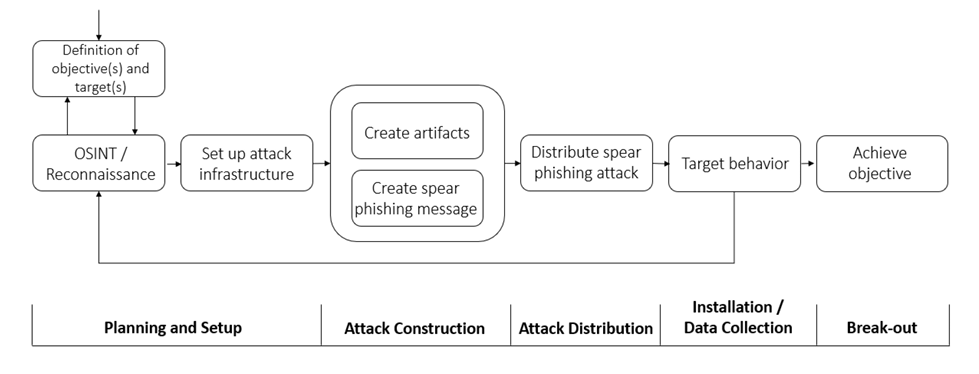
\includegraphics[width=0.75\linewidth]{phishingproc.png}
    \caption{Figure 2.1: The spearphishing process}
    \label{fig:placeholder}
\end{figure}

\subsection{Spearphishing Process}
Spearphishing attacks typically follows a multi-phase process. This model, shown in Figure 2.1, combines stages from social engineering attack frameworks with the phishing attack lifecycle.
\subsubsection{Planning and Setup:}
\begin{itemize}
    \item The attacker defines the objective and selects the target(s). Next,Open-Source Intelligence (OSINT) is gathered to learn more about the target. Based on new insights, the attacker may refine their objectives or target list. Then, the necessary infrastructure-such as phishing websites, fake domains, or malware-is prepared.
\end{itemize}
\subsubsection{Attack Construction:}
\begin{itemize}
    \item The spearphishing message is crafted using the information gathered, tailored to the targets and aligned with the attack goals. Additional artifacts like malware or phishing sites may be created during this phase.
\end{itemize}
\subsubsection{Attack Distribution}
The message is sent to the targets via chosen communications channels (e.g., email, SMS, or social media).
\subsubsection{Installation / Data Collection:}
\begin{itemize}
    \item The attacker monitors how targets respond-such as by clicking links, entering credentials, downloading malware, or replying. This stage reflects the attacker's ability to collect data or gain initial access.
\end{itemize}
\subsubsection{Break-Out:}
\begin{itemize}
    \item If the objective is achieved, the attacker may proceed with further exploitation or clean up traces, collecting more intel, or reattempting delivery.
\end{itemize}

\subsection{Spearphishing Techniques}
A spearphishing technique is defined as a non-trivial method used to perform part of the spearphishing process. "Non-trivial" means the attacker deliberately chooses the methods from a set of options based on the context or objective.

Examples include:
\begin{itemize}
    \item Using OSINT tools fo reconnaissance
    \item Choosing SMS as the delivery channel (smishing)
\end{itemize}

\subsection{Attack Context Element}
To understand spearphishing in practice, it is not enough to study the techniques used-we must also consider the attack context in which decisions are made.

The attack context includes all information available to the attacker that could influence their method selection. An attack context element is any specific piece of that information.

Examples of context elements:
\begin{itemize}
    \item Target characteristics (e.g., role, age, profession)
    \item External events (e.g., pandemics, corporate news)
    \item Pre-established infrastructure
    \item Responses from earlier phishing attempts
\end{itemize}

These context elements can shape both which techniques are used and how they are implemented.

\subsection{Techniques and Context Elements}
Research into spearphishing techniques and contextual factors is extensive, covering everything from fake social media profile creation to hosting phishing websites on the dark web, and using persuasion principles in phishing messages.

However, most reviews and surveys focus on defensive strategies, such as:

\begin{itemize}
    \item Semantic attack detection
    \item Phishing classification methods
    \item General phishing and spearphishing defenses
\end{itemize}

\subsection{Offensive Spearphishing in Literature}
Only a few academic studies focus on offensive spearphishing techniques—and those that do are often high-level or narrowly scoped. Rarely do they explore spearphishing in depth or in practical terms.

 \begin{itemize}
    \item Some literature review general phishing types, phishing "in the wild," or specific components such as malicious URLs, social engineering malware, and human vulnerability factors.

For example, some literature reviews examine general phishing categories, attacks observed “in the wild,” or specific technical components such as:
\item Malicious URLs
\item Social engineering malware
\item Human vulnerability factors
A small number of broader surveys include:
\item General overviews of phishing attack types, defense mechanisms, and research challenges—but with minimal detail on offensive methods
        \item Taxonomies of phishing vectors and technical tools—yet lacking real-world implementation depth
        \item Studies that focus more heavily on countermeasures than attack strategies
    \end{itemize}

Currently, there is no comprehensive detailed review of spearphishing techniques or the many contextual factors that attackers consider when choosing them. This represents a significant knowledge gap for defenders and Red Team practitioners who need to understand how spearphishing is realistically carried out.

\subsubsection{2.2.2 Spearphishing in Practice}

Studies on real-world offensive spearphishing are limited, especially those focused on \textbf{how Red Teams execute these attacks}. Most existing research examines broader Red Team concepts rather than spearphishing techniques.

Industry researchers have defined Red Teaming in commercial contexts and compared it to penetration testing, emphasizing its focus on simulating threat actor behavior rather than just identifying technical flaws.
\begin{itemize}
    \item \textbf{Cybersecurity analysts} have discussed when Red Team exercises are most useful when used to assess the security posture of an organization.
    \item \textbf{Legal and risk specialists} have proposed ways to reduce legal and reputational risks during engagements.
\end{itemize}

Some sources provide high-level overviews of Red Team engagement processes, including some general tactics and techniques. Others have conducted interviews with Red Team members and offered anecdotal insight into operational practices; however, some articles lack technical detail about the methods Red Teams use these articles to carry out spearphishing attacks or how they choose their approach based on context.

This lack of detail makes it difficult for defenders to benchmark, replicate, or improve offensive spearphishing simulations in their own organizations.

\subsection{Methodology}

This section outlines a structured approach to comparing spearphishing practices used by Red Teams with those documented in academic literature. The aim is to help defenders understand where gaps exist between theory and practice.

To structure this analysis:
RQ1 is addressed through a focused literature review of offensive spearphishing research.
RQ2 is answered through semi-structured interviews with Red Team professionals from a large consulting firm.
\textbf{RQ3} is answered by comparing the findings from RQ1 and RQ2.
The scope of each question is intentionally narrowed for clarity:
RQ1 excludes certain context elements and focuses on specific stages of the spearphishing process that are most relevant for offensive analysis.
RQ2 includes all relevant techniques and context elements but draws only from a select set of experienced Red Teamers.


\subsubsection{3.1 RQ1 – spearphishing Techniques and Attack Context Elements}

To answer RQ1, defenders should develop a \textbf{structured overview} of offensive spearphishing methods and the contextual factors that influence them. This helps identify which techniques are discussed in literature and under what conditions they are applied.

The process involves:

\begin{enumerate}
    \item Defining which techniques and context elements fall within the scope of analysis
    \item Collecting and reviewing relevant academic articles
    \item Extracting and categorizing the techniques and context elements they describe
\end{enumerate}

\subsubsection{3.1.1 Scope for the Literature Study}

Spearphishing techniques and context elements are broad concepts. Without limitations, a review of the literature would become overly large and unfocused. To keep it actionable for defenders, the scope is narrowed to:

\paragraph{\textbf{Context Elements:}}
Only \textbf{offensive-relevant context elements} are included.

Elements tied to \textbf{defensive actions or mitigation} by targets are excluded.

\subsection{\textbf{Spearphishing Techniques}}
Only techniques relevant to \textbf{specific stages} of the spearphishing process are included.

Two criteria guide inclusions:
\begin{itemize}
    \item Is the step unique to spearphishing (not just general cyberattacks)?
    \item Would Red Teams benefit from applying these techniques?
\end{itemize}

These criteria were validated in consultation with a Red Team subject matter expert.

\subsubsection{3.1.2 Included Steps and Rationale}

\textbf{In Scope:}

\textbf{1. Select Targets:}
Critical to spearphishing. Selecting high-value or vulnerable targets is a key challenge for Red Teams.

\textbf{2. Gather OSINT:}
Collecting publicly available data is essential to personalize attacks. Techniques for OSINT are included. General reconnaissance methods (for example, calling the target or technical scanning) are excluded.

\textbf{3. Create Artifacts (excluding malware):}
Techniques for building believable phishing content (e.g., fake PDFs, cloned login portals) are in scope. Malware creation is excluded as it applies more broadly beyond spearphishing.

\textbf{4. Craft Spearphishing Message:}
Message generation is key to spearphishing success. This includes structure, tone, pretexting methods, and the use of psychological principles.

\textbf{5. Distribute the Attack:}
Methods of delivery, such as email, SMS, messaging platforms, and others are included.

\textbf{Out of Scope:}

\textbf{1. Define Objectives:}
In Red Teaming, objectives are usually predefined by the client, not chosen by the attacker.

\textbf{2. Plan / Resource Attack:}
Resource planning is not spearphishing-specific.

\textbf{3. Set Up Infrastructure:}
Decisions here are based on tools and logistics—not useful for understanding spearphishing strategy.

\textbf{4. Target Behavior (e.g., clicking, downloading):}
These are responses to an attack, not attacker actions, and are treated as part of the \textbf{context} not the \textbf{techniques}.

\textbf{5. Collect Data and Monitor Targets:}
This step relates to persistence or post-exploitation, not spearphishing execution.

\textbf{6. Break-Out Phase:}
Actions taken after success (e.g., covering tracks, lateral movement) are dependent on broader attack goals and offer little insight into spearphishing strategy.

\subsubsection{Summary: In-Scope Spearphishing Steps}

Defenders conducting a review should focus on techniques used in the following stages of the spearphishing process:

\begin{itemize}
\item Selecting targets
\item Gathering OSINT
\item Creating artifacts (excluding malware)
\item Crafting the spearphishing message
\item Distributing the attack
\end{itemize}

\subsection{Step 3: Include Emerging Research on AI-Driven Spearphishing}
Given the rise of Large Language Models (LLMs) in crafting phishing content, defenders must also account for AI-generated spearphishing techniques.

Because this is a rapidly evolving area, traditional databases may lag in indexing relevant research. Google Scholar can be used with a search such as:
\begin{lstlisting}
    ("LLM" OR "large language model" OR "ChatGPT" OR "GPT") AND "phishing"
\end{lstlisting}

The goal is to find articles discussing:

\begin{itemize}
    \item The use of AI to automate message crafting
    \item Experimental results with LLM-generated phishing attacks
    \item Potential risks and mitigation strategies
\end{itemize}

Review titles and abstracts to filter out irrelevant results and stop once newer pages begin surfacing unrelated content.

\subsection{Step 4: Use Snowballing to Fill Gaps}
To ensure coverage is as complete as possible, defenders should review the references of all collected articles. This snowballing technique helps identify relevant sources that may not appear in keyword-based searches.

When examining references:
\begin{itemize}
    \item Look for studies cited in support of offensive techniques or context elements
    \item Prioritize articles that introduce something not already seen in earlier searches
    \item Include alternative or conflicting perspectives on spearphishing methods
\end{itemize}

When a cited paper seems relevant, scan its title, abstract, and-if necessary-its main sections to assess inclusion.

This approach gives defenders a replicable process for effectively building a detailed and up-to-date view of offensive spearphishing tactics, rooted in both foundational literature and cutting-edge developments.

\subsection{Identifying and Categorizing Techniques and Context Elements for Spearphishing}
To make the findings from academic literature useful for acute comparison with real-world Red Team practices (RQ3 with spearphishing techniques and attack context elements must first be systematically identified and categorized.

\subsubsection{Identifying Techniques and Context Elements from Literature}
From the collected articles, relevant techniques and context elements are extracted based on the definitions and scope established in Section 3.1.1. When possible, conclusions drawn in the articles about these techniques or elements are also recorded.

Determining whether something qualifies as a technique or a context element is not always that straightforward. For instance, the use of a specific OSINT tool like Maltego qualifies as a technique, but it also serves as an example of a broader method: Using OSINT tools. In such cases, the more abstract method is recorded as the primary technique, and the specific tool is noted as an example.

Where multiple examples are found for a given technique, only a representative subset is cited to keep the dataset manageable.

\subsubsection{Categorizing for Comparison with Practice}
To enable a direct and structured comparison between literature-based findings (RQ1) and real-world Red Team practices (RQ2), all identified techniques and context elements are organized into categories.This categorization process supports clarity and consistency in answering RQ3.

The process follow a hybrid approach as such:
\begin{itemize}
    \item Top-down: high-level categories are defined in advance based on the spearphishing process and context models used.
    \item Bottom-up: Subcategories are created as needed during the analysis, based on patterns that emerge from the datasets.
\end{itemize}

\subsubsection{Context Element Categories}
Context elements are sorted into three high-level groups, as such:
\textbf{1. Attacker Context}
\begin{itemize}
\item Describes characteristics or constraints specific to the attacker, such as skill level, available resources, or tools and time.
\end{itemize}
\textbf{2. Individual Target Context}
\begin{itemize}
    \item Covers attributes of a specific target, such as their job role, behavior, or digital footprint.
\end{itemize}
\textbf{3. Environmental Context}
\begin{itemize}
    \item Encompasses broader organizational and situational factors, including company culture, ongoing events (e.g., a merger or a crisis), or the pool of potential targets. For example:
    \begin{itemize}
        \item \textit{Target age} and \textit{target gender} fall under Individual Target Context and can be grouped into a subcategory such as Demographics.
    \end{itemize}
\end{itemize}

\subsubsection{Technique Categories}
Techniques are organized into five high-level categories, aligned with the spearphishing process steps defined in the literature scope (Section 3.1.1):
\textbf{1. Select Targets}
\textbf{2. Gather OSINT}
\textbf{3. Create Artifacts} (excluding malware)
\textbf{4. Craft Spearphishing Message}
\textbf{5. Distribute Attack}
Within each step performed, related techniques are grouped into subcategories as they emerge from the data. This allows defenders to trace not just \textit{what} techniques exist, but also \textit{where} in the attack lifecycle they are applied.

\subsubsection{Ensuring Consistent Categorization}
The categories are designed to be internally consistent and non-overlapping. As the review progresses, categories may be created, merged, or split to better reflect the literature.

While there may be more than one valid way to categorize the same content, consistency is maintained between the literature review and interview analysis. This ensures that the final comparison in RQ3 remains valid and meaningful-regardless of how specific groupings are structured.

\subsection{RQ2-Spearphishing Techniques and Context Elements Used in Practice}
To answer RQ2-and in support of the comparison in RQ3-this research compiles a structured overview of spearphishing techniques and attack context elements used and considered by Red Teams in real-world engagements. This overview includes concrete examples, as well as reasoning behind the selection and application of different techniques.

The data for this analysis was collected through semi-structured interviews with Red Team professionals. The sections below explain how the interview protocol was designed, how participants were selected, how interviews were conducted, and how responses were collected and analyzed.

\subsubsection{Interview Design}
The interview structure was built around two main goals:
1. To identify which spearphishing techniques and context elements Red Teams use and consider in practice (RQ2), and
2. To ensure the data can be meaningfully compared with literature findings (RQ3).

To achieve these goals, a semi-structured format was used, blending standardized questions with flexibility for deeper exploration. The interview was divided into four main sections consisting of:
\subsubsection{\textbf{1. Introductory Questions}}
These questions establish the participant's background and level of experience with spearphishing in Red Team operations. This context is important for assessing the relevance and reliability of their insights.
\textbf{2. Process-Oriented Questions}
Participants are asked to describe the overall spearphishing process they follow. This helps map out how techniques are applied in context, and ensures that the sequence of attack stages is well understood.
3. Technique-Specific Questions
These questions dive into each subsequent stage of the spearphishing process-such as target selection, OSINT gathering, message crafting, and attack distribution-and ask what techniques are typically used. These questions are also designed to surface the context elements that Red Teamers consider when choosing or modifying their approach.
\textbf{4. Campaign Walkthrough}
Participants are asked to walk through a realistic spearphishing campaign from beginning to end. This provides:
\begin{itemize}
    \item A complete view of how steps are connected in practice
    \item A way to validate earlier responses
    \item An opportunity to identify techniques or context factors that may not have come up in isolated questions
\end{itemize}

This campaign-focused question also helps detect any steps, strategies, or decision points that might not be emphasized in the literature and articles gathered.

A full list of the interview questions can be found in the Appendices section.

\subsubsection{Participant Selection}
To gather meaningful insights into real-world spearphishing practices, interview participants were selected from across the offensive security teams within DoDNIC global network. All participants had direct experience executing spearphishing campaigns in the context of Red Teaming and CCRI engagements.

In total 10 professionals and 7 international offices took part in the study. Participants ranged from senior associates with several years of hands-on experience to team leads and directors overseeing Red Team operations.

Before participating, each interviewee signed an informed consent form, which outlined:
\begin{itemize}
    \item The purpose of the interview
    \item The voluntary nature of participation
    \item How their data would be recorded, used, and stored

\end{itemize}

\subsubsection{Interview Process}
Paticipants received the informed consent from ahead of time, ensuring full transparency about the process and goals of the interview. Each interview lasted approximately 50 minutes, with audio recorded for transcription and analysis-except in two cases:
1. One participant preferred not to be recorded; their answers were written down during the session.
2. Another participants had limited availability, resulting in a 25-minute interview that focused on a smaller subset of techniques.

The interviews followed the semi-structured format outlined in Section 3.2.1, with space for:
\begin{itemize}
    \item Follow-up questions for clarification
    \item Additional prompts to explore specific techniques or decision-making contexts

\end{itemize}

Because of time constraints, not all process steps could be explored equally in every interview. Instead, each session focused in greater depth on specific phases of the spearphishing process-based on the participant's expertise and whether they introduced techniques or context elements not yet discussed in other interviews.

After each session:
\begin{itemize}
    \item Interview were transcribed manually to maintain control over interpretation.
    \item In some cases, answers were lightly paraphrased to streamline transcription efforts- without altering original meaning.
    \item All recordings and transcripts were stored securely on a DoD-issued GFE (Government Furnished Equipment) laptop and subsequently deleted after analysis was completed, in accordance with data handling protocols specific to the agency or target organization.
\end{itemize}

\subsubsection{Data Analysis}

The interview data was analyzed with two main objectives in mind:
1. To reconstruct the spearphishing process as it is carried out in practice by Red Teams
2. To categorize the techniques and context elements discussed by participants in a way that supports direct comparison with the literature findings (RQ3).

\subsubsection{Deriving the Practical Spearphishing Process}
The very first step in the analysis was to build a generalized spearphishing process model based on participant inputs. This model was constructed by combining the processes described across interviewees.

While individual Red Team members described variations in step order or emphasis, these differences were not critical. The goal was not to capture exact sequences (with the sound understanding that they all differ and vary), but to produce a high-level process model comparable to the one derived from literature (Figure 2.1). All techniques mentioned by participants were mapped to one or more steps in this detailed and generalized process.

\subsubsection{Categorizing Techniques and Context Elements}
To enable a structured comparison between practice (RQ2) and literature (RQ1), the existing categorization framework developed during the literature study was reused during interview analysis.
\begin{itemize}
    \item For techniques, any new steps described by Red Teamers-those not already covered in the literature-based process-were added as additional high-level categories.
    \item For context elements, the original three high-level categories (attacker context, individual target context, and environmental context) already encompassed all possible elements, so no new top-level categories were needed at that time.
\end{itemize}

\subsubsection{Identification and Classification Approach}
Techniques and context elements were identified and categorized using the same method applied during the literature review; however, with two key differences:
\textbf{1. No scope limitations were applied} during identification. All relevant techniques and context elements mentioned in interviews were included.
\textbf{2. Categorization was flexible}, but grounded in the original framework. If an item fit an existing category from the literature, it was placed there. If it related to a newly added step from the practical process, a new subcategory was created as needed.

Alongside each technique or context element, the analysis also recorded:
\begin{itemize}
    \item Examples provided by the participants (e.g., specific tools, channels, or message styles)
    \item Reasoning behind technique selection or contextual considerations (e.g., why a certain method was used for a given scenario vice another)
\end{itemize}

This approach ensured that the interview data could be compared directly to the literature-both structurally and substantively-when answering RQ3.

\subsection{RQ3-Comparing Literature and Practice}
To answer RQ3, the spearphishing techniques and attack context elements identified from literature (RQ1) and Red Team practice (RQ2) are compared using a structured three-level framework. This allows for a nuanced analysis of where, how, and why gaps or misalignments exist between research and real-world application.

\subsection{Levels of Comparison}
Differences between literature and practice are identified on the following three levels:

\textbf{1. Category-Level differences}
A category-level difference occurs when an entire category of techniques or context elements exist in one domain (literature or practice) but not in the other.
\textit{Example:} A specific phase of the spearphishing process used by Red Teams that was not discussed in the literature review.
\textbf{2. Technique-Level Differences}
A technique-level difference appears when a specific technique or context element is found in one domain but missing in the other-within an existing shared category.
\textit{Example:} The use of LinkedIn automation tools to gather OSINT may appear in interviews but not in academic sources.
\textbf{3. Reasoning-Level Differences}
A reasoning-level difference is noted when a technique or context element is found in both domains, but the rationale or implementation differs.
\textit{Example:} Literature might describe a method as effective based on experimental results, while practitioners dismiss it due to operational constraints or risk of detection.

\subsection{Scope Considerations and Interpretation}
\begin{itemize}
    \item Category-level differences that result solely from the limited scope of the literature review are acknowledged but not analyzed in detail, as they reflect methodological boundaries rather than practical insight gaps.
    \item Technique-level differences are all noted; however, discussion is limited to cases where the reason for the discrepancy can be clearly inferred-either from the academic literature or the interviewee's responses.
    \item Reasoning-level differences are the most common. While many minor deviations are expected, only notable or strategic differences are highlighted and discussed. These are prioritized when they offer:
    \begin{itemize}
        \item Opportunities to improve Red Team methods
        \item Insightful directions fo future research
        \item Evidence of evolving attacker behavior not yet reflected in literature
    \end{itemize}
\end{itemize}

This structured comparison not only highlights what is missing from current academic discourses but also identifies which specific techniques are most relevant for defenders looking to align threat behaviors into simulations with real-world attacker behaviors applied.

\subsection{Spearphishing Techniques and Context Elements in the Literature}
This section presents the results of the literature review aimed at answering \textbf{RQ1: What spearphishing techniques and attack context elements are discussed in the literature?}

The review process was based on three structured searches:
\begin{itemize}
    \item \textbf{Search 1 (Scopus, literature reviews and surveys)}
    \begin{itemize}
        \item 128 articles identified
        \item 38 articles read
        \item 90 excluded (e.g., focused solely on defenses, unrelated to phishing, inaccessible, or improper languages)
    \end{itemize}
\item \textbf{Search 2 (Scopus, primary spearphishing research)}
\begin{itemize}
    \item 236 articles identified
    \item 39 articles read
\end{itemize}
\item \textbf{Search 3 (Google Scholar, AI-generated phishing)}
\begin{itemize}
    \item 1060 results
    \item First 50 scanned
    \item 12 relevant articles read
\end{itemize}
\end{itemize}

Additional relevant articles were found using Google dorks and snowballing (e.g., reviewing references in included articles. In total, 133 articles were used to extract techniques, context elements, and relevant conclusions.
\begin{figure}
    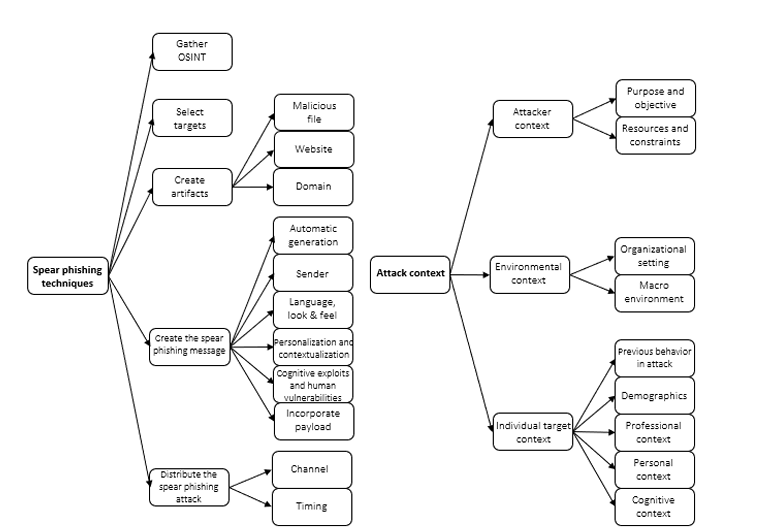
\includegraphics[width=0.75\linewidth]{spearphishing-techniques.png}
    \caption{Figure 4.1: Categorizations of spearphishing techniques and attack context elements within scope discussed in the literature Caption}
    \label{fig:placeholder}
\end{figure}
The figure above summarizes the categorization of spearphishing techniques and attack context elements found across the literature, based on the scoped phases of the spearphishing attack process methodology.

The results are organized into two main parts:
1. 4.1.1: Spearphishing techniques
2. 4.2.1: Attack context elements
Each section begins with a summary table of identified items, followed by discussion.

\subsection{Spearphishing Techniques}
Most techniques found in the literature could be clearly mapped to one of the five scoped stages of the spearphishing process: selecting targets, gathering OSINT, creating artifacts, crafting messages, and distributing the attack.

\subsection{Cross-Cutting Technologies}
Two techniques stood out as especially important because they span multiple stages of the spearphishing attack process:
\textbf{1. Structured Methodologies for Red Teamers}
A structured spearphishing attack methodology aims to provide a step-by-step guide through target selection, OSINT gathering, and message creation. The goal is to help less experienced Red Teamers run more effective simulations. While not a novel technique in and of itself, the structural approach to combining methods across steps is valuable for operational consistency and training.
\textbf{2. Phishing Tools and Automation Kits}
Tools like \textbf{Gophish, King Phisher,} and \textbf{SPToolkit} automate large portions of the phishing process, such as:
\begin{itemize}
    \item Cloning full websites
    \item Customizing and tailoring phishing emails targeted at specific identified target individuals
    \item Capturing user interactions (e.g., clicks, credentials)
\end{itemize}
These tools significantly reduce setup time and increase scalability, making them especially relevant for Red Teams and defenders simulating persistent threats.

 \subsection{Methods to Gather OSINT}

\textbf{1. Technique:}
\begin{itemize}
    \item Gather a high quantities of information
\end{itemize}
\textbf{2. What Information to Gather:}
\begin{itemize}
    \item Collect a broad profile of the target to identify exploitable traits, affiliations, and behaviors
\textbf{3. Where to Look (Online Resources)}
    \item Google, Bing, Hunter.io, Pipl.com, BeenVerified, IntelX
\end{itemize}

\textbf{1. Technique:}
\begin{itemize}
    \item Search for specific information

\end{itemize}
\textbf{2. What Information to Gather:}
\begin{itemize}
    \item Job titles, contact details, addresses, calendar links, contacts list, internal lingo, personal interests
\end{itemize}
\textbf{3. Where to Look (Online Resources)}
\begin{itemize}
    \item LinkedIn, ZoomInfo, RocketReach, GitHub, Reddit, Company blogs, Facebook
\end{itemize}

\subsection{How to Search for OSINT}
\textbf{1. Technique:}
\begin{itemize}
    \item Use OSINT tools and automate and structure collections from multiple sources
\textbf{2. Tools Used:}
\item Maltego, SpiderFoot, Recon-ng, Shodan, FOCA, Datasploit
    \end{itemize}

\textbf{1. Technique:}
\begin{itemize}
    \item     Use a VPN (Virtual Private Network) to cloak source location and bypass geo-restrictions
\textbf{2. Tools Used:}
\item NordVPN, ProtonVPN, Mullvad
    \end{itemize}

\textbf{1. Technique:} 
\begin{itemize}
    \item Use a Large Language Model (LLM) to extract, summarize, or generate intelligence using open-text sources
\textbf{2. Tools Used:}
\item ChatGPT, Claude, Perplexity.ai (used on data scraped via OSINT)
    \end{itemize}

\subsubsection{Where to Search for OSINT}

\textbf{Social Media Platforms:}
\begin{itemize}
    \item Personal information, photos, behaviors, activity patterns
\textbf{Where to Look:}
\item LinkedIn, Twitter / X, Facebook, Instagram, Snapchat, TikTok, Mastodon, open directories
    \end{itemize}

\textbf{Corporate Websites:}
\begin{itemize}
    \item Employee directories, press releases, organizational changes
\textbf{Where to Look:}
\item Company official websites and homepages, press pages, investor relations section, open directories
    \end{itemize}

\textbf{Other Public Sources:}
\begin{itemize}
    \item External appearances, blogs, event attendance, dev activity
\textbf{Where to Look:}
\item GitHub, Medium, Substack, Stack Overflow, Eventbrite, SlideShare, open directories
    \end{itemize}

\textbf{Data from Breaches (pastebins and dumpsites):}
\begin{itemize}
    \item Leaked passwords, internal communications, emails
\textbf{Where to Look:}
\item HaveIBeenPwned, DeHashed, BreachForum (dark web), Leak-Lookup
    \end{itemize}

\textbf{Physical Location Information:}
\begin{itemize}
    \item Physical access points, schedules, printed materials
\textbf{Where to Look:}
\item Google Maps, Street View, Yelp, LinkedIn events, IRL ("In-Real-Life") physical recon
    \end{itemize}

OSINT Gathering: Practical Techniques and Red Team Applications
Gathering OSINT is a foundational step in identifying attack context elements for spearphishing. Evidence shows that the amount and type of information collected can significantly impact the success and outcome of a planned and targeted attack. In a role-playing study, it was found that participants who received more detailed information about their targets wrote spearphishing emails that were nearly three times more effective than those who received minimal information. While high-volume data collection is time-consuming, it becomes especially valuable in whaling attacks-targeting high-value individuals such as executives-where attackers often analyze not only the target but also their social and professional networks.

Red Teams can also benefit from collecting specific types of information to tailor attacks. For example, impersonating a colleague or crafting malware tailored to the software a target uses reqiures highly specific OSINT; however, the literature also shows diminishing returns in some cases, such as no significant difference in susceptibility between messages personalized with only demographic data and those using a deeper context like personal interests or professional background.

To gather OSINT efficiently, various tools are available at your disposal. General-purpose frameworks like \textbf{Maltego}, \textbf{theHarvester}, and \textbf{Metagoofill} automate broad data collections while more targeted tools like \textbf{Truecaller} help retrieve personal contact information from phone numbers, and cross-linked scrapes social media profiles. \textbf{IntelliSpect} is another tool designed to combat multiple OSINT capabilities. Given that OSINT activities can raise detection flags, attackers often use VPNs to remain anonymous during collection efforts and phases. Alternatively, Large Language Models (LLMs) can assist in summarizing publicly available content or answering queries about a target's digital presence and its environment.

OSINT sources can be grouped into several categories. Social media platforms are especially rich in data-often public, persistent, and under-monitored. Beyond basic details like name, role, and education, researchers have shown that social platforms can reveal implicit attributes, such as a target's personality type, social habits, and emotional tone. Social data can even be aggregated to infer birthdays, educational history, or organizational trends, such as staff turnover.

Organizational websites also provide high-valued data, including employee directories, job titles, roles and responsibilities, and company news. Even overlooked elements-such as metadata from uploaded files or developer comments embedded in HTML-can offer clues for crafting convincing phishing content. References to recent internal events (e.g., town halls or product launches) can further increase message credibility.

In addition, public infrastructure data can be leveraged. \texttt{WHOIS/RWHOIS} databases provide information on domain ownership and network blocks, while platforms such as \textbf{Shodan}, Censys, \textbf{and} \textbf{ZoomEye} reveal exposed systems and IoT through active internet scanning. Attackers may also use \textit{Google Dorking} to uncover unsecured devices or forgotten web pages, and services like the Internet Archive to access cached versions of pages that have since been removed or restricted.

Data breach repositories represent another critical OSINT source. Sites like Have I Been Pwned? expose leaked credentials, internal emails, and organizational structure from past breaches. Lastly, physical reconnaissance still plays a huge role. Attackers may choose to visit company sites to gather physical OSINT-from visible screens to discarded documents or badge access points-highlighting that the threat landscape extends beyond digital domains.

For Red Teams, effectively applying these OSINT methods enables more authentic, targeted spearphishing campaigns. They key is balancing the breadth of data with relevance, ensuring every piece of gathered intelligence directly contributes to the plausibility and impact of the simulated spearphishing attack.

The next subsection will discuss the context elements that influence target selection and implementation.

\subsection{Target Selection Techniques and Their Application in Red Team Spearphishing Campaigns}
Selecting the right targets is a critical component of a successful spearphishing campaign, and the literature offers several strategies defenders can apply. Each method aligns with different attacker goals-ranging from maximizing effectiveness to minimizing detection risk.

One approach is to prioritize targets whose relationships and technical environments are already known.  Knowing a target's colleagues or commonly used software allows attackers to impersonate trusted individuals or craft malware tailored to known platforms. Access to more information results in more persuasive spearphishing emails, supporting the value of high-volume OSINT for target selection.

Another widely used strategy is to select targets based on their relevance to attack objectives. This becomes especially important in whaling attacks, where attackers focus on high-value individuals such as senior executives. These individuals often control or access privileged systems and sensitive data, justifying the greater effort required to craft tailored messages.

Red teams can also benefit from selecting targets based on susceptibility to phishing. The literature identifies multiple factors that affect how likely a person is to fall for an attack:

Job roles and habits: Roles involving frequent external communication increase susceptibility, especially when the phishing message mimics a normal interaction pattern. If opening emails or clicking links is a routine task, users are more likely to do so reflexively.
Seniority and experience: Junior employees are found to be more vulnerable than senior staff, possibly due to less familiarity with internal communication norms or lower exposure to phishing training and awareness.
Psychological state: Temporary factors such as mood can influence susceptibility. For example, people in a happy emotional state are more prone to phishing than those in neutral or sad moods.
Technical aptitude, confidence, and experience: Users with higher self-efficacy, more web experience, and better security knowledge are generally less likely to be deceived.
Training history: Prior exposure to simulated or real phishing attacks reduces a person's likelihood of falling for future attempts.

While many characteristics correlate with susceptibility, the literature also shows mixed or contradictory findings for some:

Workload: Higher workload can increase susceptibility, but may also lead to ignoring the phishing message entirely.
Education: Some studies find lower education levels correlate with higher risk, but others find no significant relationship.
Culture: Cultural dimensions such as power distance can affect susceptibility. In cultures where people are more deferential to authority, phishing that impersonates individuals of authority may be more effective; however, trust and cultural traits do not show consistent effects across all studies.
Personality traits: Traits like extraversion and conscientiousness have been linked to increased susceptibility, though again, findings are inconsistent across studies.
Gender and age: There is no clear consensus. Some studies report women to be more susceptible, while others find no difference. Age-related findings also vary: some studies show younger users are more susceptible, others find older users to be at a higher risk, and some report no clear correlation at all.

In addition to susceptibility, likelihood to report a phishing attempt is another useful filter for Red Teams. Selecting targets who are less likely to report the attempt can increase campaign success. Individuals with a higher self-efficacy and cybersecurity awareness are more likely to report phishing attempts, and studies show that individuals with high altruism and perceived social responsibilities (subjective norms) also report more often than not.

By incorporating factors-susceptibility, likelihood of reporting, and alignment with objectives-Red Teams can more effectively simulate realistic adversarial behaviors and test organizational resilience. These selection strategies allow for smarter targeting, especially in high-stakes or limited-scoped environments like executive phishing simulations.

\subsection{Target Selection: What Defenders Should Know}
Understanding how attackers-or Red Teams acting in their place-select targets is critical for strengthening an organization's resiliency and defense strategy. The literature outlines a range of techniques used to identify vulnerable individuals, and knowing these can help defenders both improve awareness training efforts and design more effective internal testing.

One common method is selecting targets whose workplace relationships and technologies are already exposed online. If an attacker knows who a target collaborates with or what software they use, they can craft more credible phishing lures, for example, impersonating a coworker or sending a malicious file disguised as a shared document. In this context, defenders should be especially aware of information leakage through social media, job postings, and publicly available documents of interest.

Attackers also prioritize targets for whom large amounts of information are available. Individuals who craft phishing emails using rich target data produced messages that were significantly more convincing. Defenders should assume that anyone with a large digital footprint is a potential entry point and ensure such individuals receive enhanced awareness training.

Another key insight is that target selection often aligns with attacker objectives. In high-effort campaigns-such as whaling attacks- attackers focus on those with access to privileged systems or sensitive data, such as executives and department heads. Organizations should recognize that the most senior individuals may be among the most attractive targets and ensure they are not exempt from security training or monitoring.

In addition to strategic value, attackers often choose individuals based on susceptibility to phishing. This includes psychological, behavioral, and role-based factors. For instance:
\begin{itemize}
    \item People in roles that involve frequent external communication (e.g., HR, finance, or sales) are often more exposed and more accustomed to opening emails and attachments.
    \item Routine behaviors-such as habitually checking emails-can make employees more vulnerable.
    \item Junior employees may be less familiar with internal communications processes, patterns, or phishing awareness programs, making them easier to deceive.
\end{itemize}

Defensive teams should also be aware that susceptibility is influenced by factors like technical confidence, security training, and even emotional state. People with lower computer self-efficacy or little security experience are generally more vulnerable, while mood can also play a role-those in a positive emotional state may let their guard down more easily.

The literature, however, presents mixed findings on attributes such as education, age, and gender. While some studies find lower education correlates with higher susceptibility, others find no link. Similarly, while some research suggest younger adults are more vulnerable, others find that older employees or those with heavy workloads are more likely to fall for a phishing attack. Cultural traits like deference to authority or trust can also have an influence in certain regions or organizations.

As stated previously, one often overlooked factor in target selection is the likelihood that someone will report a phishing attempt. Some employees are more proactive when it comes to reporting suspicious messages-especially those with higher self-efficacy, a strong security mindset, or a sense of social responsibility. From a defensive standpoint, this means employees who are less likely to report could represent both a detection blind spot and a greater risk if compromised.

Taken together, these insights suggest defenders should not apply a one-size-fits-all model for phishing awareness. Instead, security programs should:
\begin{itemize}
    \item Tailor security awareness training based on roles and digital exposure
    \item Monitor for high-risk behaviors and exposure
    \item Ensure senior leaders are included in security awareness and simulated exercises
    \item Evaluate employee likelihood to report phishing as part of incident response readiness efforts
\end{itemize}

By understanding how attackers choose their targets, defenders can better anticipate adversarial behaviors, design smarter awareness campaigns, and improve the realism and effectiveness of internal Red Team simulations.

\section{Crafting Malicious Files: Defensive Implications}
From a defender's view, understanding how attackers create malicious files helps in both anticipating real-world threats and improving internal Red Team simulations. One common method is manipulating the appearance of file types to make them appear harmless. For example, attackers may change the icon of an executable (EXE) file to resemble a Word document, image, or PDF, misleading users into trusting and opening it. Similarly, attackers can use file extension spoofing, like the right-to-left override technique, to make dangerous files appear benign (e.g., "\texttt{.exe}" rendered as "\texttt{.doc}").

The choice of file type also plays a critical role. Office documents with macros, even to this day, remain one of the most frequently abused formats, as they can execute code when opened and are widely used in corporate environments. PDFs are another commonly exploited format due to their ubiquity and the relative ease with which they can be spoofed or weaponized. Other techniques involve compressing executable files inside ZIP archives and asking users to unzip and run them, or attaching malicious HTML files that use auto-redirects (e.g.,  via the meta-refresh tag) to take targets and redirect them to fraudulent phishing websites. It has been noted that HTML attachments can be even more effective than placing a suspicious-looking link directly in the email.

Defenders should ensure their secure email gateways, EDR solutions, and user security awareness programs are equipped to detect and flag such techniques. Particularly, users should be trained to distrust unexpected attachments-especially from unknown senders-and systems should monitor for suspicious file behaviors such as macro execution or unexpected outbound traffic after file interaction.

\subsection{Crafting Phishing Websites: Defensive Implications}
Malicious websites are not just for credential theft; they are often designed to add legitimacy to the overall phishing narrative. For example, attackers may clone or fabricate websites tied to fake companies, especially if the phishing message refers to them as partners, vendors, or clients. Using a tool like \textbf{HTTrack}, attackers can clone a real corporate site with subtle changes to create such a ruse.

Cloning logon pages of the target's actual organization is another common tactic, especially when the goal is to steal credentials. Attackers frequently use phishing frameworks or tools like Gophish or King Phisher to achieve this. Recent work also shows how attackers use LLMs to help create phishing sites by prompting them to generate cleaned-up, stripped-down clones of login pages that exclude detection-prone elements.

For defenders, this highlights the importance of continuously monitoring for domain impersonation (especially "lookalike" domains), deploying anti-phishing protections like DMARC, and conducting regular Red Team simulations that include cloned login pages to increase realism and believability.

To evade detection, attackers often protect phishing sites in ways that make them harder to take down or identify/attribute. Hosting on the dark web is one strategy, as it hides critical metadata such as DNS and \texttt{WHOIS} records. Another technique is fast flux, where a domain's IP address rapidly changes, making it harder to denylist or detect in time. Fast flux can dramatically increase a phishing site's lifespan-from an average of 62 hours to over 190 hours. Though defenses against fast flux exist, such as network-based anomaly detection, they are not always universally implemented.

Finally, attackers may embed malicious logic or payloads in non-text elements such as images, Flash, scripts, or ActiveX objects. These bypass many detection methods based on textual or HTML structure analysis and raises the need for defenders to adopt more advanced detection system solutions that include visual similarity analysis and behavioral monitoring of websites accessed via internal networks.

\subsection{Creating Malicious Files: Attacker Perspective}
In targeted spearphishing campaigns, malicious file attachments are powerful tool to gain initial access, especially when crafted to bypass both technical defenses and user suspicions. One widely used tactic is to manipulate how the file appears to their victim. This includes changing the file icon to mimic a more trustworthy format. Beyond visual deception, attackers often apply file extension spoofing by using the right-to-left override techniques to make dangerous files appear benign in file explorers or email clients.

Choosing the right file type to exploit is critical. Office documents with enabled macros are a go-to method, given that they are commonly used in corporate communications and can execute embedded scripts when opened. PDFs are another prime target: they are universally accepted and can be weaponized easily. Some attackers also deliver zipped EXE files to encourage victims to extract and run them, taking advantage of lax content filtering. A more covert approach involves attaching HTML files that auto-redirect uses to malicious websites via the meta-refresh tag-often outperforming direct URL placement in fraudulent emails.

These techniques are chosen not only for their success rates but also based on the target organization's defensive posture. If standard file types like .exe are likely to be flagged or blocked, attackers can pivot to formats that appear more legitimate. Tools used to create these payloads are often customized and tested against sandboxed environments ensuring delivery and execution.

\subsection{Creating Phishing Websites: Attacker Perspective}
Malicious websites serve a dual role in spearphishing: they capture credentials or deploy payloads, and they lend credibility to the phishing narrative. A common tactic is cloning the website of a real or fabricated organization. For instance , an attacker might clone the website of a well-known supplier, tweak the branding slightly, and present it as a legitimate partner referenced in the phishing message.

Cloning the target organization's actual login page is another high-yielding tactic, particularly when aiming for credential harvesting. This can be done using tools like HTTrack, or integrated features in phishing kits such as Gophish or King Phisher. To avoid copying defensive artifacts or unwanted JavaScript, some attackers can use LLMs to assist in selectively replicating relevant components of a website while cleaning up potentially revealing details.

To increase the lifespan and resilience of phishing infratructures, attackers can deploy a number of defensive evasion techniques. Hosting on the dark web helps to hide DNS records, HTTPS certificates, and other metadata commonly used in domain reputation systems. Another method, as explained above is \textbf{fast flux}, where the phishing domain's IP address rotates frequently to avoid detection and denylisting-extending a phishing site's lifetime from just over 2 days to more than 8 days on average. Attackers may also embed content (such as images or scripts) rather than using static text or HTML, which can help evade signature-based and ML-based phishing detection systems.

Ultimately, attackers tailor these website creation strategies to the specific context of the spearphishing campaign-factoring in target profile and dossier, organizational defenses, and the sophistication level of the payload delivery. Incorporating these techniques helps maintain stealth, maximize believability, and achieve initial objectives faster in Red Team operations or in real-world attacks.

\subsection{Acquiring a Phishing Domain}
To increase the realism of phishing campaigns, attackers often acquire domain names that closely resemble legitimate ones. A common tactic is \textbf{typosquatting}, which involves small alterations to the official domain name—such as omitting characters (\verb|wwwexample.com|), swapping letters (\verb|www.examlpe.com|), substituting characters (\verb|www.examp1e.com|), duplicating characters (\verb|www.exaample.com|), or using hyphens (\verb|www-example.com|). These variants can deceive users with minimal scrutiny. Tools like \verb|dnstwist| help automate the generation of deceptive domain variants and quickly identify available ones to register for phishing use.

Attackers also leverage user trust in \textbf{HTTPS certificates}, even when issued to malicious domains and that users are more likely to click and interact with sites that display HTTPS—even when the domain name is suspicious—making it advantageous for attackers to obtain TLS certificates and serve phishing content over secure channels.

\subsubsection{Generating Spear Phishing Messages Automatically}

Automation can significantly scale and personalize spear phishing efforts. One of the simplest approaches is \textbf{template-based messaging}, where dynamic fields such as name, role, or department are populated using available target data. Tools such as Gophish support this level of customization.

More advanced methods use \textit{Natural Language Generation (NLG)} to produce semi-personalized content based on public data. This technique enables campaigns that fall somewhere between generic phishing and highly customized spear phishing, such as "community-targeted" phishing.

The emergence of \textbf{Large Language Models (LLMs)}—like ChatGPT—has opened new avenues for crafting convincing phishing emails. LLMs can generate emails in the tone and structure expected within a target's organizational or social context. Attackers use \textit{prompt engineering} to bypass ethical filters, applying techniques such as typos, string obfuscation, payload splitting, or creating fictional scenarios to get the model to output malicious content. Tools such as \textbf{PrompInject} even automate prompt injection strategies that manipulate LLM outputs for spear phishing or pretext generation.

\subsubsection{Crafting a Sender Identity}
Establishing a credible sender identity is a cornerstone of spear phishing success. One such approach is to \textit{impersonate someone known to the target}, such as a colleague, supervisor, or friend. Research has shown that targets are dramatically more likely to trust and act on messages that appear to come from familiar sources. Even in role-play experiments, impersonating a co-worker was up to 26 times more effective than impersonating a commercial brand.

Alternatively, impersonating \textit{someone unknown to the target} can be useful when contextually appropriate—such as a job applicant emailing HR with a fake CV.

Attackers employ various \textit{technical methods to spoof sender identity. }If access to a legitimate internal account is available (via prior compromise), \textit{internal spear phishing} or lateral movement can occur, leveraging existing trust and prior conversations. If not, attackers may use \textbf{email spoofing}, exploiting the lack of authentication in SMTP. Tools can check for protections like DMARC; if spoofing is blocked, attackers can fall back on \textbf{typosquatted domains} registered specifically for impersonation purposes. Even personal email accounts (e.g., Gmail) can be used with pretexts like “sent from iPhone” to justify unusual sending behavior.

In social media-driven campaigns, attackers often create fake or cloned profiles to establish trust and rapport with unsuspecting potential targets. These profiles can be built entirely from scratch or generated by duplicating an existing individual's account-reusing profile photos, employment information, and connections to mimic legitimacy-and hell, some dark web ChatGPT models can automatically generate one for you! All in all, this tactic is commonly referred to as \textit{"catfishing."}

A catfished profile is an online account created under a false identity, often using fabricated personal details and either fake or stolen photographs. Such profiles are used to deceive others, frequently for purposes such as financial fraud, romantic manipulation, or broader social engineering objectives. The term "catfishing" can refer both to the profile itself and to the act of creating and maintaining the fraudulent online persona.

You are probably wondering. \textit{"...well, what is the difference between a cloned site,a site that is using impersonation, and one that is a catfish?"}

Well, these three overlap in concept but differ in \textit{target, medium,} and \textit{intent}-in cybersecurity and social engineering they are considered distinct tactics. Let us examine this briefly.

\subsection{1. Cloned Site}
What it is:
A complete copy of a legitimate website, usually hosted on a different domain, designed to look and behave exactly like the original.
Goal:
Trick users into entering credentials, financial information, or other sensitive data (phishing) by exploiting trust in the original site's design.
Key Traits:
Replicates layout, branding images, and text of a legitimate site.
Often delivered via malicious links in emails, SMS (smishing), or social media.
May include typosquatting in the domain name (e.g., \texttt{paypa1.com} instead of \texttt{paypal.com}).
Example:
A fake banking portal that is visually identical to the real bank's site but sends entered credentials to an attacker-controlled server.

\subsection{2. Impersonation Site (or Brand Impersonation)}
What it is:
A site that does not necessarily clone the original in full or in its entirety but one that uses brand names, logos, trademarks, or corporate identity to appear affiliated with the real entity.
Goal:
Create a perception of legitimacy to sell fake products, distribute malware, collect leads, or mislead customers.
Key Traits:
May not be an exact copy-often a modified or partial information.
Relies on \textit{brand association} more than pixel-perfect replication.
Sometimes used in \textit{Business Email Compromise (BEC)} attacks and partner scams.
Example:
A site that sells counterfeit merchandise using a near-identical logo and color scheme of a popular sportswear brand.

\subsection{Catfish (Social Media Impersonation)}
What it is:
A fake social media profile built to impersonate a real person or create an entirely fictional identity. The term hails from romance scams but also applies to professional networking and espionage contexts.
Goal:
Build trust and rapport with individuals or groups to influence, defraud, extract information, or facilitate future cyberattacks (e.g., spearphishing).
Key Traits:
Focus is on the \textit{persona}, not a website.
May reuse stolen photos, work histories, and social connections.
Success depends on human trust rather than website traffic.
Example:
A LinkedIn profile claiming to be an executive at a real company, used to connect with employees and later send malicious job-related documents.

\subsection{Key Differences at a Glance}

\begin{table}
    \centering
    \begin{tabular}{cccc}
         Aspect&  Cloned Site&  Impersonation Site& Catfish (Social Media)\\
         Medium&  Website&  Website& Social media platform\\
         Accuracy&  Pixel-perfect copy&  Partial imitation / branding mimic& Mimics a person's online identity\\
         Primary Goal&  Credential theft / phishing&  Brand exploitation, fraud, malware& Social engineering, relationship building\\
         Delivery&  Links in emails, SMS, ads&  Search results, ads, targeted outreach& Connection requests, DMs\\
         Trust Vector&  Visual similarity to legit site&  Brand recognition& Personal trust and social proof\\
    \end{tabular}
    \caption{Caption}
    \label{tab:placeholder1}
\end{table}
\section{Red Team vs. Blue Team-Site \& Profile Impersonation Tactics}

\begin{table}
    \centering
    \begin{tabular}{ccc}
         Attack Type\&  Red Team (Attacker) \& Blue Team (Defender) Perspective\\
         Cloned Site\&  Creation: Use tools like HTTrack, wget, or custom scripts to copy HTML/CSS/JS from the legitimate site. Modify form actions to send credentials to an attacker-controlled backend.
Exploitation: Host on a lookalike domain (typosquatting or homoglyph attacks). Distribute via spearphishing or whaling campaigns, SMS, or malicious ads.
Evasion: Use HTTPS with free TLS certs (e.g., Let's Ecnrypt) to appear legitimate. Employ geofencing to limit visibility to target region.\& Detection: Monitor for typosquatted domains and suspicious SSL certificates using brand monitoring services (e.g., DNSTwist, PhishLabs).
Prevention: Implement DMARC, DKIM, and SPF to reduce phishing email success. Use user education campaigns to help staff identify mismatched domains.
Response: Submit DCMA takedown requests to hosting providers and domain registrars. Update web Content Security Policies (CSPs) to block external forms.\\
         Impersonation Site\&  Creation: Build a partial copy or a newly designed site that uses stolen brand assets (logos, fonts, color schemes). May host fake job listings, fake products, or malware downloads.
Exploitation: Leverage black hat SEO poisoning, malvertising, or email campaigns to drive traffic. May impersonate a partner portal or supplier login.
Evasion: Keep site content "similar enough" to avoid automated plagiarism detection. Use anonymized WHOIS info and offshore hosting using a "bullet-proof ISP."\& Detection: Use brand monitoring services to track misuse of trademarks and logos. Search for suspicious domains with partial matches (e.g., <brand>-secure.com).
Prevention: Register common domain variants to block attackers. Watermark key brand assets where feasible.
Response: Issue legal takedowns for IP / trademark violations. Coordinate with ad networks to block malvertising.\\
         Catfishing Profile\&  Creation: Set up a fake social media profile using stolen or AI-generated profile pictures, fabricated bios, and false employment / education / history. Connect with target's real contacts to build credibility and believability& \\
    \end{tabular}
    \caption{Caption}
    \label{tab:placeholder2}
\end{table}



\subsection{Methods to Personalize and Contextualize the Spearphishing Message}
Spearphishing relies heavily on crafting messages that appear natural and inconspicuous within the target's environment. Personalization and contextualization techniques aim to make the email blend into the recipient's context and appeal directly to their interests or expectations-factors shown to significantly affect success rates. It has been studied that messages aligned with the target's situational context reduce cognitive scrutiny, making deceltion indicators less noticeable.

The degree of personalization often correlates with the value of the target. Since tailoring messages demands time, effort, and resources, attackers weigh the level of targeting against the potential payoff. High-value campaigns, such as whaling, justify deep \textit{"hypercontextualization,"} where extensive information is gathered during reconnaissance and footprinting stages before composing the message. Inserting details such as the recipient's name, their organization, and a known sender identity increases click rates fivefold compared to generic emails, or sloppily-built messages.

Topic choice also influences susceptibility. Some themes have been categorized into \textit{"life domains"} and found legal-related topics as having had the highest success rate (6.7%), while finanical topics were the lowest at j1.1/%. Simply matching the toopic to the target's known interestes has produced the highest open rates-course registration emails reached 54.4/% compared to a 27.2/% average. A well-crafted subject line can further boost engagement, as in the 2011 RSA breach, where "2011 Recruitment Plan" was used to lure employees.

Interestingly, it has been studied that no significant difference in susceptibility between attacks personalized only with the demographic data and those incorporating broader personal / professional details; however, attackers with more background knowledge still wrote more effective messages, likely due to an enhanced "theory of mind"-the ability to anticipate the target's behaviors based on their thoughts and emotions.

\subsection{Methods to Shape the Language, Look, and Feel of the Message}
Language accuracy and style can reinforce authenticity. Higher success rates have been reported when attackers spoke the target's primary language, with a 1.76x improvement over non-native speakers. Grammatical correctness also matters, as poor writing is often used by recipients to detect phishing red flags. Style consistency with the impersonated sender's usual tone further boosts credibility and believability.

Visual design elements also play a role in that an attacker can include legitimate-looking company brand logos making emails harder to detect by the target. Some attackers replace the body text with inline images, bypassing text-based spam filters while maintaining a professional appearance.

\subsection{Methods to Incorporate Cognitive Exploits of Human Vulnerabilities}
More times than not, attackers often borrow from psychology, exploiting "human vulnerabilities," or "human hacking" much like attackers exploit system flaws. These cognitive exploits are drawn from frameworks like

 
















